\problemname{The Fish Game}
You are playing the fish game. You are a fish that must eat smaller fish but must never
get eaten by larger fish. The fish never change size. You get points for each fish you eat and naturally you want
as many points as possible.

The playing field can be seen as a grid with $H$ rows (numbered from $1$ to $H$) but an unlimited number of columns. You are
in column $x=0$ and can only move vertically (up and down). The other fish never move vertically
but start in a certain column $x>0$ and float at constant speed to the left (toward your column). 

All fish (including you) have width $1$ cell. Your height is $7$. There are three other types of fish: ``small'' with height $3$,
``medium'' with height $5$, and ``large'' with height $9$. The fish have different speeds. Each second you can move one cell
up or down (or stay still). In the same time a small fish moves $1$ cell, a medium fish $2$ cells, and a large
fish $3$ cells to the left. You choose at which height level your fish starts, but note that your \emph{entire} fish
must always be within the playing field.


A fish can eat fish that are smaller than itself. You can thus eat fish of size $3$ and $5$, earning $10$
and $20$ points respectively. But fish of height $9$ will eat you, and you must watch out for them. If you get
eaten you lose. To make it fair who eats whom, the mermaid Arashiel has decided that the following happens in each discrete
time step:
\begin{enumerate}
  \item You make your move (move up, down, or stay).
  \item Large fish advance three steps, medium fish advance two steps, and small fish advance one step.
  \item Large fish eat medium and small fish (or you) if they are in the same column and overlap vertically (at least one shared cell).
  \item Medium fish that survived eat small fish if they are in the same column and overlap vertically.
  \item You eat small and medium fish if they are in your column ($x=0$) and overlap vertically.
\end{enumerate}

\section*{Input}

The first line contains two integers, $N$ ($1 \leq N \leq 50\,000$), the number of fish, and $H$ ($20 \leq H \leq 1\,000$),
the height of the field. 

Then follow $N$ lines, one for each fish. Each line starts with a letter, \texttt{L}/\texttt{M}/\texttt{S},
indicating whether the fish is small, medium, or large. Then follows the column $x$ where the fish starts ($2 \leq x \leq 10^{16}$),
and the row $y$ that is the fish's middle cell (always chosen so that the entire fish fits within the interval $[1, h]$).
The three values are separated by spaces.

Additionally:
\begin{itemize}
  \item
    No fish in the input will overlap either fully or partially (initially).
  \item
      The $x$-coordinate of each fish will always be even. For the largest
      fish size it will also always be divisible by 3. This is
      because we want all collisions to occur at integer coordinates.
  \item
    You will always be able to avoid being eaten, i.e. the game always
    has a solution.
\end{itemize}

\section*{Output}
Output a single line with a single integer, the number of points you get if you play the game optimally.

\section*{Scoring}
Your solution will be tested on a set of test groups.
To earn points for a group, you must pass all test cases in that group.

\noindent
\begin{tabular}{| l | l | l |}
  \hline
  \textbf{Group} & \textbf{Points} & \textbf{Constraints} \\ \hline
  $1$   & $20$       & $N \leq 1000$, $H \leq 50$, $x \leq 10\,000$ \\ \hline
  $2$   & $20$       & $H \leq 50$, no fish eat each other \\ \hline
  $3$   & $20$       & $H \leq 50$, medium fish never eat small fish \\ \hline
  $4$   & $20$       & $H \leq 50$ \\ \hline
  $5$   & $20$       & No additional constraints. \\ \hline
\end{tabular}

\section*{Explanation of Samples}
\begin{figure}[h!]
    \centering
    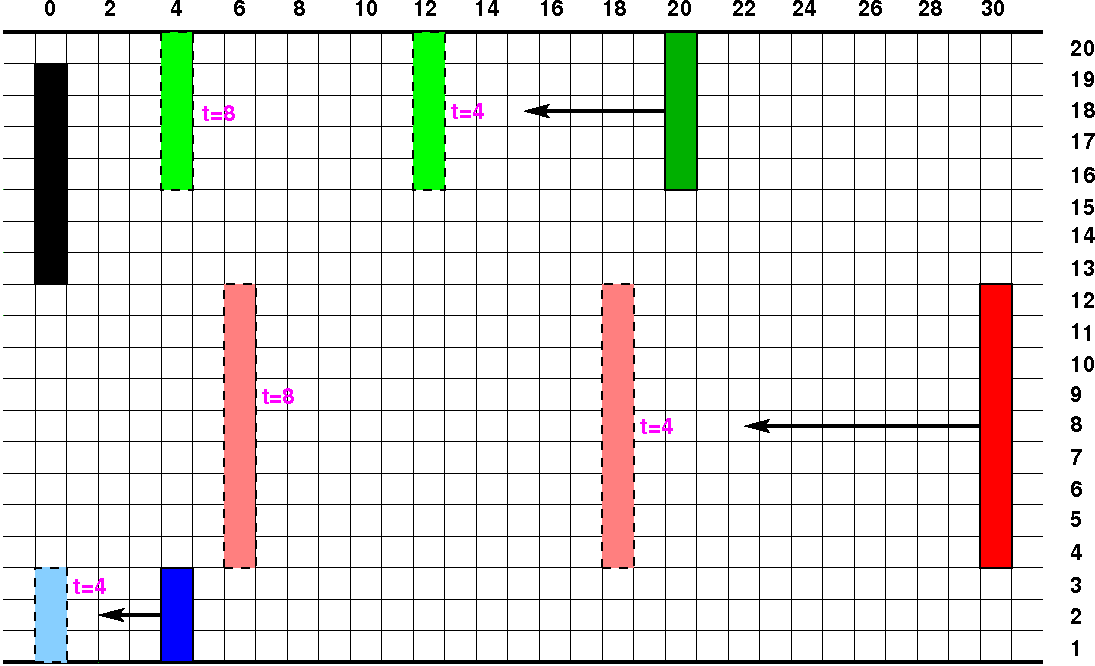
\includegraphics[width=0.75\textwidth]{fiskspelet.png}\\
\caption{The situation in sample 1}
\label{fig:sample1}
\end{figure}
\noindent
A possible solution to the first example is shown in Figure~\ref{fig:sample1}.
The solid colored rectangles
show the fish's starting positions and the dashed rectangles show
their positions after $4$ and $8$ seconds respectively. The black rectangle
shows one of several optimal starting positions for you. In this case you can
simply stand still and wait for the green medium fish.

\begin{figure}[h!]
    \centering
    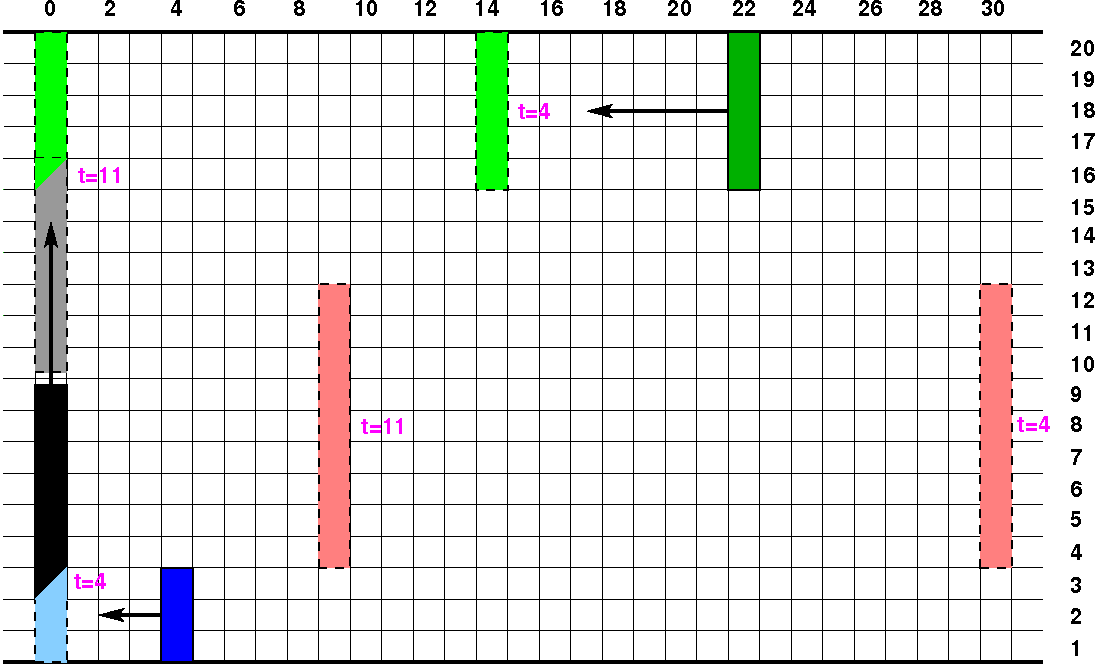
\includegraphics[width=0.75\textwidth]{fiskspelet2.png}\\
\caption{The situation in sample 2}
\label{fig:sample2}
\end{figure}
A possible solution to the second example is shown in Figure~\ref{fig:sample2}.
The black rectangle shows where you must be at time $t=4$ seconds when you eat the blue
small fish (it is fine to also have this as the starting position). The
shared cell indicates that the fish overlap on this cell. Then
you must move at full speed upward to be able to eat the green
medium fish at $t=11$ (your position is then shown by the gray dashed
rectangle). Finally you must continue upward to escape the
red large fish which reaches your column at $t=14$ (this would be too
messy to show in the figure).
